% !TEX TS-program = pdflatex
% !TEX encoding = UTF-8 Unicode

% This is a simple template for a LaTeX document using the "article" class.
% See "book", "report", "letter" for other types of document.

\documentclass[11pt]{article} % use larger type; default would be 10pt

\usepackage[utf8]{inputenc} % set input encoding (not needed with XeLaTeX)

%%% Examples of Article customizations
% These packages are optional, depending whether you want the features they provide.
% See the LaTeX Companion or other references for full information.

%%% PAGE DIMENSIONS
\usepackage{geometry} % to change the page dimensions
\geometry{a4paper} % or letterpaper (US) or a5paper or....
% \geometry{margin=2in} % for example, change the margins to 2 inches all round
% \geometry{landscape} % set up the page for landscape
%   read geometry.pdf for detailed page layout information

\usepackage{graphicx} % support the \includegraphics command and options

% \usepackage[parfill]{parskip} % Activate to begin paragraphs with an empty line rather than an indent

%%% PACKAGES
\usepackage{booktabs} % for much better looking tables
\usepackage{array} % for better arrays (eg matrices) in maths
\usepackage{paralist} % very flexible & customisable lists (eg. enumerate/itemize, etc.)
\usepackage{verbatim} % adds environment for commenting out blocks of text & for better verbatim
\usepackage{subfig} % make it possible to include more than one captioned figure/table in a single float
% These packages are all incorporated in the memoir class to one degree or another...

%%% HEADERS & FOOTERS
\usepackage{fancyhdr} % This should be set AFTER setting up the page geometry
\pagestyle{fancy} % options: empty , plain , fancy
\renewcommand{\headrulewidth}{0pt} % customise the layout...
\lhead{}\chead{}\rhead{}
\lfoot{}\cfoot{\thepage}\rfoot{}

%%% SECTION TITLE APPEARANCE
\usepackage{sectsty}
\allsectionsfont{\sffamily\mdseries\upshape} % (See the fntguide.pdf for font help)
% (This matches ConTeXt defaults)

%%% ToC (table of contents) APPEARANCE
\usepackage[nottoc,notlof,notlot]{tocbibind} % Put the bibliography in the ToC
\usepackage[titles,subfigure]{tocloft} % Alter the style of the Table of Contents
\renewcommand{\cftsecfont}{\rmfamily\mdseries\upshape}
\renewcommand{\cftsecpagefont}{\rmfamily\mdseries\upshape} % No bold!

%%% END Article customizations

%%% The "real" document content comes below...

\title{Brief Article}
\author{The Author}
%\date{} % Activate to display a given date or no date (if empty),
         % otherwise the current date is printed 

\begin{document}
\maketitle

\section{a) Berechnen Sie die $\epsilon$-Hülle für jeden Zustand.}
$\epsilon$-Hülle von q$_{0}$ = \{q$_{0}$,q$_{1}$,q$_{2}$\}\\
$\epsilon$-Hülle von q$_{1}$ = \{q$_{1}$\}\\
$\epsilon$-Hülle von q$_{2}$ = \{q$_{2}$\}\\
$\epsilon$-Hülle von q$_{3}$ = \{q$_{0}$,q$_{1}$,q$_{2}$,q$_{3}$\}\\


\section{b) Geben Sie die Übergangstabelle $\delta_{E}$ an.}
 \begin{tabular}{c|c|c}
  $Q_{\epsilon}$&0&1\\
  \hline
    $\emptyset$ &$\emptyset$&$\emptyset$\\
  $\to$ q$_{0}$ &\{q$_{2}$,q$_{3}$\}&\{q$_{0}$,q$_{3}$\}\\
  q$_{1}$ & $\emptyset$ & \{q$_{3}$\} \\
  q$_{2}$ & \{q$_{3}$\} & \{q$_{3}$\}\\
  $\ast q_{3}$ & \{q$_{2}$,q$_{3}$\} & \{q$_{0}$,q$_{3}$\}\\
 \end{tabular}
\section{Konstruieren Sie ein DEA D }
\subsection{Geben Sie der Startzustand  $Q_{D}$ an}
\{q$_{0}$,q$_{1}$,q$_{2}$\}
\subsection{Geben Sie der Zustände  $Q_{D}$ als Potenzmenge von $Q_{\epsilon}$ an}
 $Q_{D}$ = \{
q$_{0}$,
q$_{1}$,
q$_{2}$,
q$_{3}$,
\{q$_{0}$,q$_{1}$\},
\{q$_{0}$,q$_{2}$\},
\{q$_{0}$,q$_{3}$\},
\{q$_{1}$,q$_{2}$\},
\{q$_{1}$,q$_{3}$\},
\{q$_{2}$,q$_{3}$\},
\{q$_{0}$,q$_{1}$,q$_{2}$\},
\{q$_{0}$,q$_{1}$,q$_{3}$\},
\{q$_{0}$,q$_{2}$,q$_{3}$\},
\{q$_{1}$,q$_{2}$,q$_{3}$\},
\{q$_{0}$,q$_{1}$,q$_{2}$,q$_{3}$\}
\}
\subsection{Geben Sie die akzeptierten Zustände $F_{D}$ von $Q_{D}$ an}
$F_{D} =$\{q$_{3}$,\{q$_{0}$,q$_{3}$,\},\{q$_{1}$,q$_{3}$,\},\{q$_{2}$,q$_{3}$,\},
\{q$_{0}$,q$_{1}$,q$_{3}$\},
\{q$_{0}$,q$_{2}$,q$_{3}$\},
\{q$_{1}$,q$_{2}$,q$_{3}$\},
\{q$_{0}$,q$_{1}$,q$_{2}$,q$_{3}$\}\}
\subsection{ Bestimmen Sie die Übergänge des DEA D}
\begin{tabular}{c|c|c}
$Q_{D}$&0&1\\
\hline
$\emptyset$ &$\emptyset$&$\emptyset$\\
q$_{0}$ &$\ast$\{q$_{2}$,q$_{3}$\}&$\ast$\{q$_{0}$,q$_{3}$\}\\
q$_{1}$ & $\emptyset$ &$\ast$\{q$_{3}$\} \\
q$_{2}$ &$\ast$\{q$_{3}$\} &$\ast$\{q$_{3}$\}\\
$\ast q_{3}$ & \{q$_{2}$,q$_{3}$\} &$\ast$\{q$_{0}$,q$_{3}$\}\\
\{q$_{0}$,q$_{1}$\}&$\ast$\{q$_{2}$,q$_{3}$\}&$\ast$\{q$_{0}$,q$_{3}$\}\\
\{q$_{0}$,q$_{2}$\}&$\ast$\{q$_{2}$,q$_{3}$\}&$\ast$\{q$_{0}$,q$_{3}$\}\\
$\ast$\{q$_{0}$,q$_{3}$\}&$\ast$\{q$_{2}$,q$_{3}$\}&$\ast$\{q$_{0}$,q$_{3}$\}\\
\{q$_{1}$,q$_{2}$\}&$\ast$q$_{3}$&$\ast$q$_{3}$\\
$\ast$\{q$_{1}$,q$_{3}$\}&$\ast$\{q$_{2}$,q$_{3}$\}&$\ast$\{q$_{0}$,q$_{3}$\}\\
$\ast$\{q$_{2}$,q$_{3}$\}&$\ast$\{q$_{2}$,q$_{3}$\}&$\ast$\{q$_{0}$,q$_{3}$\}\\
$\to$\{q$_{0}$,q$_{1}$,q$_{2}$\}&$\ast$\{q$_{2}$,q$_{3}$\}&$\ast$\{q$_{0}$,q$_{3}$\}\\
$\ast$\{q$_{0}$,q$_{1}$,q$_{3}$\}&$\ast$\{q$_{2}$,q$_{3}$\}&$\ast$\{q$_{0}$,q$_{3}$\}\\
$\ast$\{q$_{0}$,q$_{2}$,q$_{3}$\}&$\ast$\{q$_{2}$,q$_{3}$\}&$\ast$\{q$_{0}$,q$_{3}$\}\\
$\ast$\{q$_{1}$,q$_{2}$,q$_{3}$\}&$\ast$\{q$_{2}$,q$_{3}$\}&$\ast$\{q$_{0}$,q$_{3}$\}\\
$\ast$\{q$_{0}$,q$_{1}$,q$_{2}$,q$_{3}$\}&$\ast$\{q$_{2}$,q$_{3}$\}&$\ast$\{q$_{0}$,q$_{3}$\}\\
   \end{tabular}
\subsection{ Bestimmen Sie die Übergänge des DEA D vom Startzustand aus }
\begin{tabular}{c|c|c}
$Q_{D}$&0&1\\
\hline
$\emptyset$ &$\emptyset$&$\emptyset$\\
$\ast$\{q$_{0}$,q$_{3}$\}&$\ast$\{q$_{2}$,q$_{3}$\}&$\ast$\{q$_{0}$,q$_{3}$\}\\
$\ast$\{q$_{2}$,q$_{3}$\}&$\ast$\{q$_{2}$,q$_{3}$\}&$\ast$\{q$_{0}$,q$_{3}$\}\\
$\to$\{q$_{0}$,q$_{1}$,q$_{2}$\}&$\ast$\{q$_{2}$,q$_{3}$\}&$\ast$\{q$_{0}$,q$_{3}$\}\\
\end{tabular}
\subsection{Zeichnen Sie das Zustandsdiagramm des DEA D.}
$\ast$\{q$_{0}$,q$_{3}$\} $\widehat{=}$ C\\
$\ast$\{q$_{2}$,q$_{3}$\} $\widehat{=}$  B\\
$\to$\{q$_{0}$,q$_{1}$,q$_{2}$\} $\widehat{=}$ A\\
\begin{figure}
	\centering
	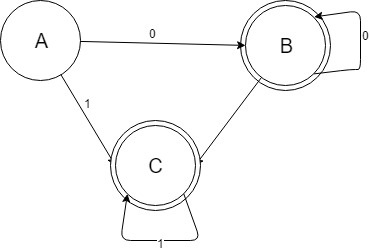
\includegraphics{zustand.jpg}
	\caption{Zustandsdiagramm}
\end{figure}
\end{document}
